\section{State-of-the-Art Methods}

Phần này trình bày chi tiết bốn phương pháp đại diện cho sự phát triển của lĩnh vực Saliency Detection từ traditional methods đến deep learning approaches. Mỗi phương pháp được phân tích theo cùng một khung để đảm bảo tính so sánh và đối chiếu.

\subsection{Spectral Residual (2007)}

\subsubsection{Nguyên lý}

Spectral Residual \cite{sr_2007} dựa trên giả thuyết rằng các vùng salient tương ứng với những thành phần không thể dự đoán được trong phổ tần số của ảnh. Phương pháp này xuất phát từ quan sát rằng phổ log của ảnh tự nhiên thường có tính chất dự đoán được, trong khi các vùng salient tạo ra các "residual" trong phổ này.

\begin{itemize}
    \item \textbf{Input (Ảnh Gốc):} $I \in \mathbb{R}^{H \times W \times 3}$. Để tối ưu, ảnh thường được resize về $64 \times 64$ nhằm loại bỏ chi tiết nhiễu cao tần.
    \item \textbf{Output (Bản đồ Dự đoán):} $\mathcal{S} \in \mathbb{R}^{H \times W \times 1}$, đại diện cho độ nổi bật của từng pixel trong miền không gian sau khi đã lọc bỏ các thành phần lặp lại trong miền tần số.
    \item \textbf{Ground Truth (Bản đồ Thực):} $S \in \mathbb{R}^{H \times W \times 1}$, là các vùng salient được xác định trước để đánh giá hiệu suất.
\end{itemize}

\textbf{Thuật toán hoạt động dựa trên các phương trình toán học cốt lõi sau:}\\
- \textbf{Chuyển đổi sang miền tần số:} Sử dụng biến đổi Fourier (FFT) để tách biên độ và pha của ảnh $I(x,y)$:
\begin{equation}
\mathcal{F}[I(x,y)] = \mathcal{A}(f) \cdot e^{i\mathcal{P}(f)}
\end{equation}
- \textbf{Tính toán phổ Log (Log-spectrum): }Chuyển biên độ sang thang đo logarit để phân tích cấu trúc phổ:
\begin{equation}
\mathcal{L}(f) = \log(\mathcal{A}(f))
\end{equation}
- \textbf{Trích xuất phần dư phổ (Spectral Residual): }
\begin{equation}
\mathcal{R}(f) = \mathcal{L}(f) - [h_n(f) * \mathcal{L}(f)]
\end{equation}
- \textbf{Tái cấu trúc trong miền không gian:} Kết hợp phần dư phổ $\mathcal{R}(f)$ với thông tin pha ban đầu $\mathcal{P}(f)$ và thực hiện biến đổi Fourier ngược (IFFT):
\begin{equation}
\mathcal{S}(x,y) = |\mathcal{F}^{-1}[e^{\mathcal{R}(f) + i\mathcal{P}(f)}]|
\end{equation}
- \textbf{Làm mượt:} 
\begin{equation}
\text{Saliency Map} = g(x,y) * \mathcal{S}(x,y)^2
\end{equation}

\noindent \textbf{Trong đó:}
\begin{itemize}
    \item $I(x,y)$: Ảnh đầu vào cần xử lý.
    \item $\mathcal{F}[\cdot], \mathcal{F}^{-1}[\cdot]$: Phép biến đổi Fourier và biến đổi Fourier ngược.
    \item $\mathcal{A}(f)$: Phổ biên độ (Amplitude spectrum) của ảnh, tuân theo quy luật $1/f$.
    \item $\mathcal{P}(f)$: Phổ pha (Phase spectrum), chứa thông tin cấu trúc không gian và được giữ nguyên trong quá trình xử lý.
    \item $\mathcal{L}(f)$: Phổ Logarit (Log-spectrum), biểu diễn biên độ trên thang log.
    \item $h_n(f)$: Bộ lọc trung bình cục bộ (Local average filter) kích thước $n \times n$.
    \item $\mathcal{R}(f)$: Phần dư phổ (Spectral Residual), đại diện cho phần thông tin của ảnh sau khi loại bỏ dư thừa.
    \item $g(x,y)$: Bộ lọc làm mịn Gaussian (Gaussian filter) với $\sigma=8$.
\end{itemize}
\subsubsection{Phương pháp}
\noindent Pipeline của phương pháp bao gồm 5 bước chính:
\begin{enumerate}
    \item \textbf{Chuyển đổi Miền Tần số:} Chuyển ảnh sang miền tần số bằng FFT.
    \item \textbf{Phân tích Phổ Log:} Tính toán phổ log biên độ.
    \item \textbf{Tính Toán Phần Dư:} Loại bỏ thành phần dư thừa (redundant) bằng cách lấy phổ log trừ đi phổ đã được làm mượt.
    \item \textbf{Tạo Bản đồ Độ Nổi bật:} Kết hợp phần dư phổ với thông tin pha (phase spectrum) ban đầu để tái tạo ảnh trong miền không gian.
    \item \textbf{Hậu Xử lý:} Bình phương biên độ và áp dụng lọc Gaussian để thu được bản đồ độ nổi bật cuối cùng.
\end{enumerate}

Đây là phương pháp hoàn toàn bottom-up, không sử dụng thông tin ngữ nghĩa (semantic information) hoặc đặc trưng học được (learned features), mà chỉ dựa trên các đặc tính thống kê của phổ ảnh tự nhiên.
\begin{figure}[H]
    \centering
    \caption{Ví dụ đầu ra của Spectral Residual (Input, Saliency Map Output và Ground Truth) (\cite{sr_2007})}
    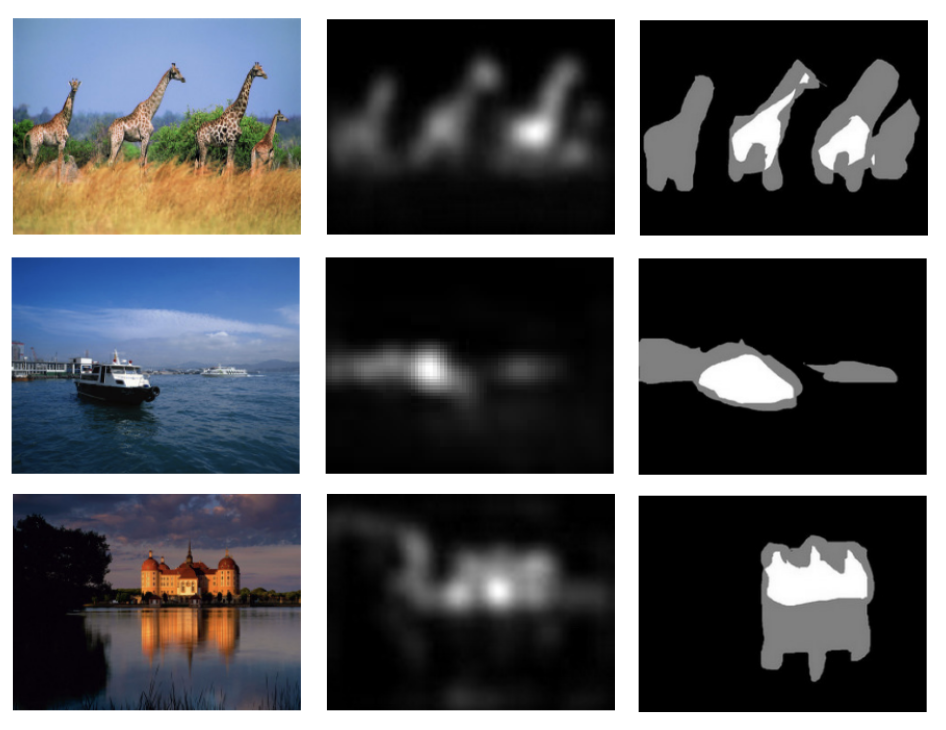
\includegraphics[width=0.8\textwidth]{img/Chapter2/OutputSR.png}

    \label{fig:output_sr}
\end{figure}

\subsubsection{Công tác Lựa chọn và Làm Dữ liệu}
\noindent Vì Spectral Residual là phương pháp không tham số, quy trình thực nghiệm tập trung vào việc đối chiếu kết quả thuật toán với sự tập trung của con người thông qua việc sàng lọc dữ liệu.

\begin{itemize}
    \item \textbf{Quy trình sàng lọc và xác định Ground Truth:}
    \begin{itemize}
        \item \textbf{Resize và lọc cao tần:} Ảnh đầu vào được resize về kích thước nhỏ (thường là \textbf{$64 \times 64$})
        \item \textbf{Mô phỏng giai đoạn tiền chú ý (Pre-attentive):} Hình ảnh phải có vật thể chủ đạo rõ ràng. Nếu người đánh giá báo cáo rằng "không thể xác định được đối tượng nằm ở đâu", ảnh đó sẽ bị loại khỏi tập dữ liệu.
        \item \textbf{Kết quả lựa chọn:} Tổng cộng có \textbf{62 hình ảnh} tự nhiên đáp ứng tiêu chuẩn "tiền chú ý" được giữ lại để kiểm tra.
        \item \textbf{Dữ liệu đánh giá (Ground Truth):} Trong bài báo này, Ground Truth được xác định bởi \textbf{đánh giá thủ công của con người (Human Annotation)}. Tác giả yêu cầu các đối tượng tham gia xác định vùng nổi bật nhất trong ảnh, thay vì sử dụng thiết bị Eye-tracking (thiết bị theo dõi ánh mắt thường dùng trong các nghiên cứu sau này).
    \end{itemize}

    \item \textbf{Chỉ số đo lường metrics riêng:}\\
    - Hit Rate (HR): Tỉ lệ vùng nổi bật do mô hình dự đoán trùng khớp với vùng mà đa số người quan sát cùng xác nhận.
    \begin{equation} HR = P(x \in R_m \mid x \in R_a) = \frac{Area(R_m \cap R_a)}{Area(R_a)} \end{equation}
    - False Alarm Rate (FAR):Tỉ lệ vùng mô hình dự đoán là nổi bật nhưng thực tế không có người quan sát nào khoanh vùng.
    \begin{equation} FAR = P(x \in R_m \mid x \notin R_a) = \frac{Area(R_m \cap \bar{R}_a)}{Area(\bar{R}_a)} \end{equation}

    \item \textbf{Nguyên lý tối ưu (Trade-off):} 
    Một phương pháp được coi là hiệu quả khi đạt được ``Hit Rate (HR) cao nhất tại một mức False Alarm Rate (FAR) chấp nhận được (thấp)". Điều này chứng minh thuật toán có khả năng tập trung đúng vào vật thể mà không bị đánh lừa bởi các yếu tố nền.
    Spectral Residual đạt performance khá tốt trên các metrics traditional:
\end{itemize}

\subsection{Performance}
\textbf{Kết quả định lượng :}
\begin{table}[H]
\centering
\caption{Cấu hình thực nghiệm và Kết quả định lượng (\cite{sr_2007})}
\begin{tabular}{|l|c|c|}
\hline
\textbf{Tập Dữ liệu huấn luyện} & \multicolumn{2}{l|}{N/A (Sử dụng đặc trưng thống kê $1/f$ của ảnh tự nhiên)} \\ \hline
\textbf{Cấu hình Input} & \multicolumn{2}{l|}{Resize về 64 pixel (width/height) để phù hợp visual scale } \\ \hline
\textbf{Số lượng ảnh thử nghiệm} & \multicolumn{2}{l|}{62 ảnh tự nhiên (đã loại bỏ ảnh không rõ đối tượng) } \\ \hline
\hline
\textbf{Performance Comparison} & \textbf{Hit Rate (HR)} & \textbf{Total Time (62 imgs)} \\ \hline
Spectral Residual (Our) & 0.4309 (tại FAR=0.1433) & \textbf{4.014s} \\ \hline
Itti's Method & 0.2482 (tại FAR=0.1433) & 61.621s \\ \hline
\end{tabular}
\end{table}

\textbf{Phân tích định tính:}
\begin{itemize}
    \item \textbf{Tốc độ xử lý:} Tổng thời gian xử lý 62 ảnh là 4.014s, trung bình khoảng \textbf{64ms/ảnh} (trên phần cứng thời điểm 2007).
    \item \textbf{So sánh:} Nhanh hơn gấp $\sim$15 lần so với phương pháp Itti (61.621s).
    \item \textbf{Cơ sở:} Chi phí tính toán chủ yếu nằm ở phép biến đổi Fourier (FFT) và Inverse FFT, được đánh giá là cực kỳ tiết kiệm (parsimonious).
\end{itemize}

\textbf{Đặc tính tính toán :}
\begin{itemize}
    \item Độ phức tạp thuật toán: $O(N \log N)$ với $N$ là số lượng pixel.
    \item Tổng thời gian xử lý bộ dữ liệu 62 ảnh chỉ mất 4.014s,  Itti mất tới 61.621s.
\end{itemize}

\textbf{Điểm mạnh:} 
\begin{itemize}
    \item Tính tổng quát cao (Generality): Không phụ thuộc vào đặc trưng, danh mục đối tượng hay kiến thức tiền nghiệm.
    \item Hiệu quả tính toán vượt trội, phù hợp cho các hệ thống thời gian thực.
    \item Giải quyết được vấn đề trọng số giữa các kênh đặc trưng (màu sắc, hướng...) mà các mô hình truyền thống gặp phải.
\end{itemize}


\textbf{Điểm yếu:} 
\begin{itemize}
    \item Không phát hiện được các đối tượng dựa trên cấu trúc nhận thức phức tạp.
    \item Bỏ qua tính đồng nhất về không gian (spatial homogeneity) của đối tượng, dẫn đến việc đối tượng có thể bị chia cắt (ví dụ: người và ngựa bị tách rời).
\end{itemize}
\subsubsection{Đóng góp}

Phương pháp \textbf{Spectral Residual (SR)} đóng góp chủ yếu vào \textbf{Bước 2 và Bước 3} của saliency detection pipeline.
\begin{itemize}
    \item \textbf{Bước 2 - Trích xuất Đặc trưng (Feature Extraction):} SR giới thiệu một cách tiếp cận hoàn toàn mới \textbf{dựa trên phân tích phổ tần số}, khai thác các đặc tính thống kê của ảnh tự nhiên thay vì sử dụng các đặc trưng thủ công truyền thống.
    \item \textbf{Bước 3 - Kết hợp Đặc trưng (Feature Integration):} Phương pháp này cung cấp một cơ chế hiệu quả để kết hợp thông tin từ phổ tần số nhằm xác định các vùng nổi bật, \textbf{tránh được các vấn đề về trọng số kênh đặc trưng} mà các mô hình trước đó gặp phải.
\end{itemize}

\subsubsection{Hạn chế}
\textbf{Hiểu biết ngữ nghĩa hạn chế:} Phương pháp thuần túy thống kê và không có khả năng hiểu nội dung ngữ nghĩa. Phương pháp bỏ qua tính đồng nhất về không gian của đối tượng, Hậu quả là các vật thể thường bị phân mảnh thành nhiều vùng rời rạc thay vì một khối thống nhất

\textbf{Xử lý vật thể có độ tương phản thấp:} Các vật thể có đặc tính quang phổ tương tự với nền (như động vật trong ngụy trang tự nhiên) thường bị bỏ sót hoàn toàn, làm nổi bật hạn chế trong khả năng phân biệt đặc điểm.

\textbf{Hạn chế về Visual Scale (Fixed Resolution):} Cố định kích thước ảnh đầu vào ở 64 pixel để mô phỏng thị giác sơ cấp. Việc thiếu xử lý đa tỷ lệ (Multi-scale) làm mất mát các chi tiết tần số cao.

\textbf{Không có khả năng học} Do là phương pháp phi tham số, nó không thể thích ứng hoặc cải thiện hiệu suất dựa trên dữ liệu chuyên biệt theo lĩnh vực hoặc sở thích của người dùng, do đó hạn chế khả năng ứng dụng trong các lĩnh vực chuyên ngành.

\textbf{Độ chính xác và Nhiễu:} Mặc dù HR cao hơn Itti (0.43 so với 0.24), mô hình vẫn gặp khó khăn nếu phổ tần số của đối tượng bị che lấp bởi phổ của nền.

\newpage
\subsection{SalGAN (2017)}

\subsubsection{Nguyên lý}

SalGAN \cite{salgan_2017} là một trong những pioneers trong việc apply Generative Adversarial Networks cho saliency prediction. Phương pháp này dựa trên giả thuyết rằng realistic saliency maps có thể được học thông qua adversarial training giữa generator và discriminator networks.

\begin{itemize}
    \item \textbf{Input (Ảnh Gốc):} $I \in \mathbb{R}^{H \times W \times 3}$.
    \item \textbf{Output (Bản đồ Dự đoán):} $\tilde{S} \in \mathbb{R}^{H \times W \times 1}$, được sinh ra bởi $G(I)$.
    \item \textbf{Ground Truth (Bản đồ Thực):} $S \in \mathbb{R}^{H \times W \times 1}$.
\end{itemize}

\noindent \textbf{a - Kiến trúc cơ bản của SalGAN bao gồm}:
\noindent \textbf{Generator Network - $G$:} 
\begin{itemize}
    \item Chức năng: Dự đoán $\hat{S}$ từ $I$.
    \item Kiến trúc: Encoder-Decoder tích chập (Encoder dựa trên VGG-16 đã sửa đổi).
    \item Ký hiệu Toán học:
    $$G(I): \mathbb{R}^{H \times W \times 3} \rightarrow \mathbb{R}^{H \times W \times 1}$$
\end{itemize}


\noindent \textbf{Discriminator Network - $D$:} 
\begin{itemize}
    \item Chức năng: Phân biệt Bản đồ Thực ($S$) và Bản đồ Giả ($\tilde{S}$).
    \item Input: Cặp ảnh $(I, \text{Map})$, với $\text{Map} \in \{S, \tilde{S}\}$.
    \item Ký hiệu Toán học: 
    $$D(I,  \theta_d): \mathbb{R}^{H \times W \times 4} \rightarrow [0, 1]$$
\end{itemize}

\noindent \textbf{b - Hàm mất mát}: Quá trình huấn luyện sử dụng BCE Loss cho Content Loss và kết hợp với Adversarial Loss.\\
- \textbf{Content Loss BCE}:
\begin{equation}
\mathcal{L}_{BCE}=-\frac{1}{N}\sum_{k=1}^{N}(S_{k}\log(\tilde{S}_{k})+(1-S_{k})\log(1-\tilde{S}_{k}))
\end{equation}
- \textbf{Hàm mất mát cho Discriminator ($\mathcal{D}$)}:
\begin{equation}
\mathcal{L}_{Dis}=L(\mathcal{D}(I,S),1)+L(\mathcal{D}(I,\tilde{S}),0)
\end{equation}
- \textbf{Hàm mất mát tổng cho Generator ($G$)}:
\begin{equation}
\mathcal{L}=\alpha \times \mathcal{L}_{BCE} + L(\mathcal{D}(I,\tilde{S}),1)
\end{equation}

\noindent Trong đó:
\begin{itemize}
    \item $I$: Ảnh đầu vào (Input image).
    \item $S$: Bản đồ độ nổi bật thực (Ground truth saliency map).
    \item $\tilde{S}$: Bản đồ độ nổi bật dự đoán (Predicted saliency map).
    \item $L$: Hàm mất mát Binary Cross Entropy (BCE).
    \item $\alpha = 5\times 10^{-3}$: Tham số trọng số (Weighting parameter).
    \item $L(\mathcal{D}(I,\tilde{S}),1)$: Thành phần \textbf{Adversarial Loss} giúp Generator đánh lừa Discriminator bằng cách làm cho kết quả dự đoán gần với giá trị 1 (thực).
\end{itemize}

\subsubsection{Phương pháp}
\noindent SalGAN pipeline gồm các components chính:
\begin{enumerate}
    \item \textbf{Cấu trúc xương sống của trích xuất đặc trưng}: Sử dụng pre-trained \textbf{VGG-16} network để extract hierarchical features từ input images, tận dụng transfer learning từ tập dữ liệu ImageNet.
    \item \textbf{Bộ tạo hoàn toàn tích chập (Fully Convolutional Generator)}: Chuyển đổi các lớp fully connected của VGG-16 thành các lớp convolutional để bảo toàn thông tin không gian (spatial information) và cho phép xử lý ảnh đầu vào với kích thước bất kỳ.
    \item \textbf{Huấn luyện đối kháng (Adversarial Training)}: Generator được huấn luyện để đánh lừa (fool) Discriminator, trong khi Discriminator học cách phân biệt bản đồ độ nổi bật thực ($S$) và bản đồ được tạo ra ($\tilde{S}$).
    \item \textbf{Huấn luyện đa hàm mất mát}: Kết hợp \textbf{Adversarial Loss} với \textbf{Content Loss} (BCE Loss) để đảm bảo cả tính chân thực (realism) và độ chính xác (accuracy) của bản đồ độ nổi bật.
    \item \textbf{Tinh chỉnh}: Ban đầu huấn luyện Generator chỉ với \textbf{Content Loss}, sau đó thêm dần thành phần \textbf{Adversarial Loss} để đảm bảo sự hội tụ ổn định (stable training convergence).
\end{enumerate}

Đây là phương pháp tiếp cận theo hướng \textbf{pure deep learning}, sử dụng \textbf{end-to-end learning} mà không cần các đặc trưng thủ công (hand-crafted features) hay các quy tắc heuristic.

\begin{figure}[H]
    \centering
    \caption{Ví dụ đầu ra của SalGAN (Input, Saliency Map Output và Ground Truth) (\cite{salgan_2017})}
    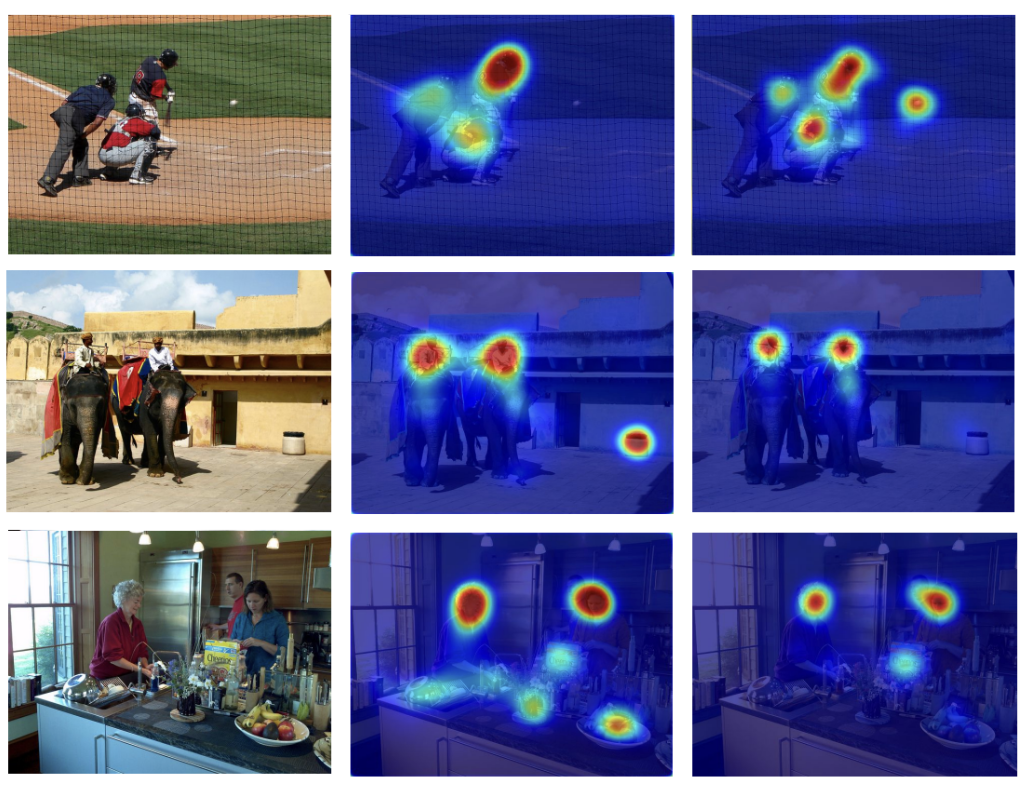
\includegraphics[width=0.8\textwidth]{img/Chapter2/OutputSalgan.png}

    \label{fig:output_salgan}
\end{figure}

\subsubsection{Công tác Lựa chọn và Làm Dữ liệu}
\begin{itemize}
    \item \textbf{Tập dữ liệu} Sử dụng bộ dữ liệu \textbf{SALICON} (10,000 ảnh huấn luyện). Các saliency maps tương ứng được tạo ra từ dữ liệu \textbf{mouse-tracking}, đóng vai trò như một nguồn dữ liệu thay thế hiệu quả cho eye-tracking chuyên dụng.

    \item \textbf{Data Augmentation:} Áp dụng kỹ thuật \textbf{random horizontal flipping} để tăng cường sự đa dạng của dữ liệu huấn luyện và giảm thiểu hiện tượng overfitting.

    \item \textbf{Giao thức Huấn luyện:}
    \begin{itemize}
        \item \textbf{Giai đoạn đầu:} Huấn luyện Generator đơn lẻ bằng cách tối ưu hóa \textbf{Content Loss} (BCE Loss) để học cách dự đoán sơ đồ độ nổi bật cơ bản.
        \item \textbf{Giai đoạn sau:} Thực hiện huấn luyện đối kháng (\textbf{Adversarial training}) giữa Generator và Discriminator bằng cách sử dụng bộ tham số được khởi tạo từ giai đoạn trước.
        \item \textbf{Optimizer:} Sử dụng \textbf{Adam optimizer} cho quá trình tối ưu hóa.
    \end{itemize}

    \item \textbf{Chiến lược Đánh giá:} Đánh giá mô hình trên tập validation của SALICON và kiểm chứng khả năng tổng quát hóa trên bộ dữ liệu MIT300.
\end{itemize}

\subsubsection{Hiệu suất}

\textbf{Kết quả định lượng:} 

\begin{table}[h]
\centering
\caption{Thông số đo lường của SalGAN trên các tập dữ liệu khác nhau (\cite{salgan_2017})}
\begin{tabular}{|l|c|c|c|c|}
\hline
\textbf{Tập dữ liệu Huấn luyện} & \multicolumn{4}{l|}{SALICON (10,000 ảnh)} \\ \hline
\textbf{Hàm mất mát} & \multicolumn{4}{l|}{BCE + Adversarial Loss} \\ \hline
\hline
\textbf{Tập dữ liệu Kiểm thử} & \textbf{AUC $\uparrow$} & \textbf{sAUC $\uparrow$} & \textbf{CC $\uparrow$} & \textbf{NSS $\uparrow$} \\ \hline
SALICON (Val) & 0.858 & 0.724 & 0.783 & 1.862 \\ \hline
MIT300 & 0.870 & 0.740 & 0.770 & 2.040 \\ \hline
\end{tabular}
\end{table}

\textbf{Phân tích định tính (Qualitative Analysis):}  Generated saliency maps trực quan chân thực và chi tiết hơn nhiều so với các phương pháp truyền thống. Nhờ Adversarial Loss, mô hình loại bỏ được hiện tượng mờ (blur) và tập trung chính xác vào các vật thể có ý nghĩa ngữ nghĩa cao (semantic objects), phản ánh đúng mẫu chú ý của con người.

\textbf{Hiệu suất trên nhiều tập dữ liệu:} Thể hiện khả năng tổng quát hóa (generalization) mạnh mẽ khi huấn luyện trên dữ liệu mouse-tracking (SALICON) nhưng vẫn đạt kết quả xuất sắc trên eye-tracking thực tế (MIT300).

\textbf{Đặc tính tính toán:} Thời gian thực hiện một lượt truyền thẳng (\textbf{Forward pass}) của SalGAN cực kỳ tối ưu, trung bình khoảng \textbf{0.02 giây (20ms)} đến \textbf{0.05 giây (50ms)} cho mỗi hình ảnh khi sử dụng GPU (thử nghiệm trên NVIDIA Titan X).

\textbf{Điểm mạnh:} 
\begin{itemize}
    \item Tạo ra bản đồ độ nổi bật chất lượng cao và chân thực.
    \item Tốc độ xử lý nhanh, đáp ứng yêu cầu thời gian thực.
    \item Khả năng tổng quát hóa mạnh mẽ giữa các tập dữ liệu (Cross-dataset).
    \item Kiến trúc dựa trên mạng VGG-16 giúp tận dụng tối đa các đặc trưng sâu.
\end{itemize}

\textbf{Điểm yếu:} 
\begin{itemize}
    \item Quá trình huấn luyện đối kháng (GAN) đòi hỏi tài nguyên tính toán lớn.
    \item Cần tinh chỉnh kỹ lưỡng tham số $\alpha$ để cân bằng giữa Content Loss và Adversarial Loss.
\end{itemize}

\subsubsection{Đóng góp}

Phương pháp SalGAN đóng góp chủ yếu vào Bước 2 và Bước 3 của saliency detection pipeline, và định hình lại cách tiếp cận học máy đầu-cuối cho bài toán này.

\begin{itemize}
    \item \textbf{Cải tiến về học đặc trưng sâu:} Thay thế hoàn toàn đặc trưng thủ công bằng các \textbf{đặc trưng phân cấp học từ CNN,} từ mức thấp đến mức ngữ nghĩa cao.
    \item \textbf{Cải tiến về học chuyển tiếp (transfer learning):} Tận dụng tri thức ngữ nghĩa từ \textit{ImageNet} để tăng chất lượng biểu diễn đặc trưng và độ ổn định huấn luyện. 
\end{itemize}
\textbf{→ Cải thiện bước 2 – Trích xuất đặc trưng.}

\begin{itemize}
    \item \textbf{Cải tiến về huấn luyện đối kháng (GAN)}: Bổ sung ràng buộc về tính chân thực thị giác cho saliency map thông qua discriminator, giúp kết quả không chỉ chính xác pixel-wise mà còn tự nhiên về mặt phân bố.
    \item \textbf{Cải tiến về học đầu-cuối (end-to-end learning)}: Hợp nhất trích xuất đặc trưng và sinh saliency map vào \textbf{một mô hình duy nhất}, loại bỏ các bước xử lý heuristic và hậu xử lý phức tạp. 
\end{itemize}
\textbf{→ Cải thiện bước 3 – Sinh bản đồ nổi bật.}

\subsubsection{Hạn chế}
\begin{itemize}
    \item \textbf{Phụ thuộc dữ liệu}: Hiệu suất phụ thuộc mạnh vào dữ liệu huấn luyện lớn; khả năng tổng quát hóa kém khi áp dụng sang miền dữ liệu khác biệt.
    \item \textbf{Huấn luyện GAN không ổn định}: Dễ xảy ra \textit{mode collapse}, đòi hỏi tinh chỉnh siêu tham số cẩn thận (đặc biệt là $\alpha$).
    \item \textbf{Tốn tài nguyên huấn luyện}: Dù suy luận nhanh, quá trình huấn luyện tiêu hao nhiều thời gian và tài nguyên tính toán.
    \item \textbf{Hạn chế đa quy mô}: Kiến trúc chủ yếu xử lý đơn quy mô, chưa tối ưu cho bối cảnh có vật thể nhiều kích thước.
    \item \textbf{Nhầm lẫn chú ý}: Chưa phân biệt rõ giữa nổi bật ngữ nghĩa và nổi bật thị giác.
\end{itemize}

\newpage
\subsection{PiCANet (2018)}
\subsubsection{Nguyên lý}

PiCANet \cite{picanet_2018} giới thiệu cơ chế Pixel-wise Contextual Attention để giải quyết hạn chế của các phương pháp trước đó trong việc mô hình hóa các mối quan hệ ngữ cảnh phụ thuộc xa (long-range dependencies). Phương pháp này dựa trên quan sát rằng đối với mỗi pixel, mạng cần lựa chọn thông tin ngữ cảnh một cách có chọn lọc thông qua các trọng số chú ý được tính toán riêng biệt cho từng vị trí.

Cơ chế cốt lõi là tính toán đặc trưng ngữ cảnh được chú ý $x_{i,j}^{att}$ cho mỗi pixel tại vị trí $(i,j)$ bằng cách tổng hợp thông tin từ tập hợp các vị trí ngữ cảnh $\mathcal{C}_{i,j}$:

- \textbf{Tổng hợp đặc trưng ngữ cảnh (Feature Aggregation):} Mạng tính toán đặc trưng ngữ cảnh được chú ý $x_{i,j}^{att}$ cho mỗi pixel tại vị trí $(i,j)$ bằng cách tổng hợp thông tin từ các vị trí trong vùng ngữ cảnh $\mathcal{C}_{i,j}$:
\begin{equation}
x_{i,j}^{att} = \sum_{n \in \mathcal{C}_{i,j}} \alpha_{i,j}^n x_n
\end{equation}

- \textbf{Tính toán trọng số chú ý (Attention Mechanism):} Trọng số $\alpha_{i,j}^n$ được xác định thông qua hàm Softmax, phản ánh mức độ quan trọng của đặc trưng tại vị trí $n$ đối với pixel đang xét $(i,j)$:
\begin{equation}
\alpha_{i,j}^n = \frac{\exp(a_{i,j}^n)}{\sum_{m \in \mathcal{C}_{i,j}} \exp(a_{i,j}^m)}
\end{equation}
Cơ chế này cho phép mô hình "may đo" (tailor) bản đồ chú ý riêng biệt cho từng pixel, kết hợp linh hoạt giữa bối cảnh toàn cục (Global) và chi tiết cục bộ (Local).

\noindent \textbf{Trong đó:}
\begin{itemize}
    \item $x_{i,j}^{att}$: Đặc trưng ngữ cảnh sau khi được áp dụng cơ chế chú ý (Attended contextual feature) tại vị trí $(i,j)$.
    \item $\mathcal{C}_{i,j}$: Tập hợp các vị trí ngữ cảnh của pixel $(i,j)$. Trong PiCANet, tập này có thể là lân cận cục bộ (Local context) hoặc toàn bộ ảnh (Global context).
    \item $x_n$: Đặc trưng đầu vào (input feature) tại vị trí ngữ cảnh $n$.
    \item $\alpha_{i,j}^n$: Trọng số chú ý (Attention weight), biểu thị mức độ đóng góp thông tin của vị trí $n$ vào việc tái tạo đặc trưng cho vị trí $(i,j)$.
    \item $a_{i,j}^n$: Điểm tương đồng (Affinity/Relevance score) thể hiện sự tương tác giữa đặc trưng tại pixel truy vấn $(i,j)$ và pixel ngữ cảnh $n$ (thường được học qua các lớp tích chập).
\end{itemize}

\subsubsection{Phương pháp}
\noindent Cấu trúc PiCANet được xây dựng dựa trên sự kết hợp giữa các module Attention và kiến trúc mạng phân cấp U-Net:

\begin{enumerate}
    \item \textbf{Xương sống trích xuất đặc trưng:} Tác giả sử dụng hai loại mạng xương sống là \textbf{VGG-16} và \textbf{ResNet-50}. Trong đó, các lớp pooling cuối cùng được loại bỏ và thay thế bằng dilated convolution nhằm duy trì độ phân giải của feature map ($28 \times 28$) trong khi vẫn mở rộng được trường thụ cảm.
    \item \textbf{Chú ý Toàn cục (Global PiCANet)::} Module này thu thập thông tin trên toàn bộ phạm vi ảnh ($H \times W$). Để tối ưu chi phí tính toán, tác giả sử dụng mạng ReNet (gồm các lớp RNN quét theo 4 hướng) để tóm tắt thông tin không gian trước khi tính toán trọng số chú ý $\alpha$.
    \item \textbf{Chú ý Cục bộ (Local PiCANet):} Tập trung vào việc tinh chỉnh chi tiết trong một cửa sổ cục bộ kích thước $D \times D$ (thường chọn $D=7$ hoặc $D=13$). Module này giúp mô hình tập trung vào các mối quan hệ không gian gần kề, đặc biệt hiệu quả trong việc làm sắc nét ranh giới vật thể.
    \item \textbf{Tích hợp Decoder (U-Net Integration)}PiCANet không đứng độc lập mà được nhúng vào các tầng của kiến trúc U-Net: 
    \begin{itemize} 
        \item Tại mỗi tầng decoder, đặc trưng từ encoder được đưa qua module PiCANet để "lọc" thông tin trước khi nối (concatenate) với đặc trưng được upsample từ tầng dưới. 
        \item Quá trình này được lặp lại đa cấp (multi-scale) để thu được kết quả cuối cùng mịn mào
        \item Cuối cùng, một lớp convolution 1x1 được sử dụng để chuyển đổi đặc trưng cuối cùng thành bản đồ độ nổi bật (saliency map).
    \end{itemize}
\end{enumerate}

\begin{figure}[H]
    \centering
    \caption{Ví dụ đầu ra của PiCANet(Input, Saliency Map Output và Ground Truth) (\cite{picanet_2018})}
    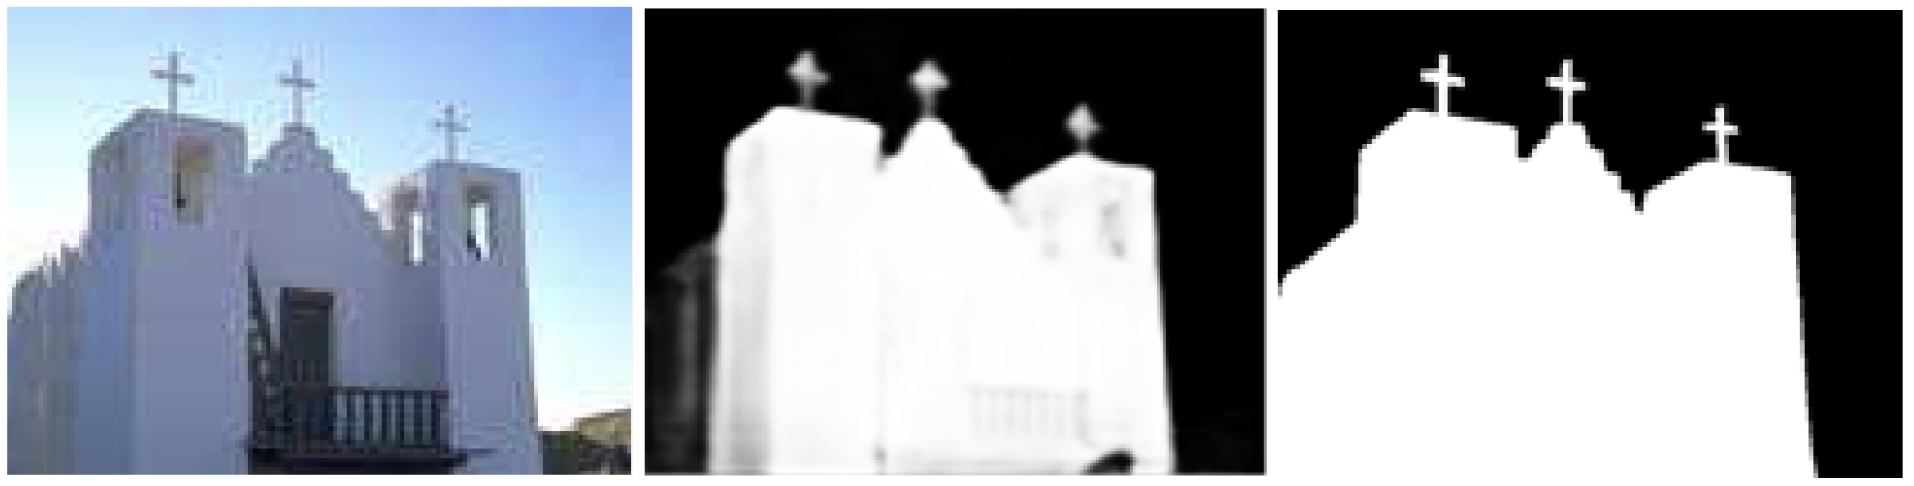
\includegraphics[width=0.8\textwidth]{img/Chapter2/OutputPicanet.png}
    \label{fig:output_picanet}
\end{figure}


\subsubsection{Công tác Lựa chọn và Làm Dữ liệu}
\begin{itemize}
    \item \textbf{Tập dữ liệu:}
    \begin{itemize}
        \item \textbf{Huấn luyện:} Sử dụng tập dữ liệu \textbf{DUTS-TR} (gồm 10,553 hình ảnh). Đây là tập dữ liệu lớn và thách thức nhất cho bài toán Salient Object Detection (SOD).
        \item \textbf{Kiểm thử:} Đánh giá trên 5 bộ benchmark phổ biến: \textbf{DUTS-TE, ECSSD, HKU-IS, PASCAL-S, và DUT-OMRON}.
    \end{itemize}

    \item \textbf{Xử lý dữ liệu:}
    \begin{itemize}
        \item Hình ảnh được resized về kích thước chuẩn $224 \times 224$ pixels đối với bản VGG. Với bản ResNet, kích thước ảnh được giữ nguyên tỷ lệ với cạnh dài tối đa là 300.
        \item \textbf{Augmentation:} Chỉ áp dụng lật ảnh ngang ngẫu nhiên theo đúng mô tả thực nghiệm trong bài báo.
    \end{itemize}

    \item \textbf{Chiến lược huấn luyện:}
    \begin{itemize}
        \item \textbf{Tối ưu:} Sử dụng giải thuật SGD với momentum 0.9 và weight decay 0.0005.
        \item \textbf{Tốc độ học:} Thiết lập $10^{-3}$ cho VGG và $10^{-2}$ cho ResNet, áp dụng chiến lược giảm dần theo hàm lũy thừa (\textit{poly policy}) với hệ số 0.9.
        \item \textbf{Hàm mất mát:} Tối ưu hóa bằng hàm Cross-entropy trên từng pixel.
    \end{itemize}
\end{itemize}

\subsubsection{Performance}
\noindent PiCANet đạt được kết quả trạng thái SOTA (tại thời điểm 2018) trên các bài toán SOD:

\textbf{Kết quả định lượng:}
\begin{table}[H]
\centering
\caption{Thông số đo lường củat PiCANet-R trên các tập dữ liệu khác nhau (\cite{picanet_2018})}
\begin{tabular}{|l|c|c|}
\hline
\textbf{Tập dữ liệu huấn luyện} & \multicolumn{2}{l|}{DUTS-TR (10,553 ảnh)} \\ \hline
\textbf{Kích thước Input} & \multicolumn{2}{l|}{300 $\times$ 300 (ResNet backbone)} \\ \hline
\textbf{Tối ưu} & \multicolumn{2}{l|}{SGD (momentum 0.9, decay 0.0005)} \\ \hline
\hline
\textbf{Tập dữ liệu kiểm thử} & \textbf{max $F_{\beta} \uparrow$} & \textbf{MAE $\downarrow$} \\ \hline
DUTS-TE & 0.825 & 0.051 \\ \hline
ECSSD & 0.917 & 0.046 \\ \hline
HKU-IS & 0.895 & 0.042 \\ \hline
DUT-OMRON & 0.739 & 0.068 \\ \hline
\end{tabular}
\end{table}


\textbf{Phân tích tốc độ (Inference time trên Titan X GPU):}
\begin{itemize}
    \item Bản PiCANet-VGG: \textbf{0.136s}.
    \item Bản PiCANet-ResNet: \textbf{0.184s}.
\end{itemize}

\textbf{Điểm mạnh:} Khả năng mô hình hóa ngữ cảnh chọn lọc cực tốt; định vị vật thể chính xác ngay cả khi vật thể có kích thước cực lớn hoặc cực nhỏ; ranh giới dự đoán sắc nét.

\textbf{Điểm yếu:} Độ phức tạp tính toán cao; tiêu tốn nhiều bộ nhớ VRAM cho các ma trận attention khi xử lý ảnh độ phân giải cao.

\subsubsection{Đóng góp}
Phương pháp PiCANet đóng góp chủ yếu vào Bước 2 và Bước 3 của saliency detection pipeline, tập trung vào việc cải thiện cơ chế mô hình hóa ngữ cảnh và chú ý trong dự đoán saliency.

\begin{itemize}
    \item \textbf{Cải tiến về cơ chế chú ý theo pixel (pixel-wise attention):} Đề xuất cơ chế chú ý được học \textbf{riêng cho từng pixel}, cho phép mỗi vị trí tự lựa chọn vùng ngữ cảnh quan trọng và bỏ qua các vùng gây nhiễu.
    \item \textbf{Cải tiến về mô hình hóa ngữ cảnh Global–Local:} Kết hợp đồng thời thông tin ngữ cảnh toàn cục (Global) và chi tiết cục bộ (Local), giúp tăng khả năng phân biệt vật thể nổi bật với nền phức tạp.
\end{itemize}
\textbf{→ Cải thiện Bước 2 – Trích xuất đặc trưng (Context-aware Feature Extraction).}

\begin{itemize}
    \item \textbf{Cải tiến về cấu trúc decoder tích hợp attention:} Nhúng các module PiCANet vào kiến trúc encoder–decoder (U-Net), cho phép lan truyền thông tin chú ý trong quá trình tái tạo saliency map.
\end{itemize}
\textbf{→ Cải thiện Bước 3 – Sinh bản đồ nổi bật.}

\subsubsection{Hạn chế}
\begin{itemize}
    \item \textbf{Sự phức tạp về tính toán (Computational Complexity):} Phép toán tính attention cho mỗi pixel có độ phức tạp bậc hai so với kích thước ảnh, gây khó khăn cho việc xử lý ảnh độ phân giải cao.
    \item \textbf{Yêu cầu bộ nhớ (Memory Constraint):} Lưu trữ các trọng số chú ý đòi hỏi dung lượng bộ nhớ lớn trong quá trình huấn luyện và dự đoán.
    \item \textbf{Sự phụ thuộc vào Backbone:} Hiệu năng của cơ chế chú ý phụ thuộc lớn vào chất lượng của các đặc trưng trích xuất từ mạng xương sống (VGG/ResNet).
    \item \textbf{Khả năng ứng dụng thời gian thực:} Với tốc độ khoảng 5-7 FPS, mô hình chưa phù hợp cho các tác vụ video yêu cầu thời gian thực khắt khe mà không có sự tối ưu hóa phần cứng.
\end{itemize}

\newpage
\subsection{U²-Net (2020)}
\subsubsection{Nguyên lý}

% \textbf{Edge Case Handling:} Architecture optimized cho typical salient object scenarios may underperform trong edge cases như transparent objects, reflections, hoặc extreme lighting conditions, indicating limitation trong \textit{robustness across diverse conditions}.
U²-Net \cite{u2net_2020} giới thiệu kiến trúc mạng hình chữ U lồng nhau hai cấp (two-level nested U-structure). Thành phần cốt lõi là khối Residual U-block (RSU), cho phép trích xuất đặc trưng đa quy mô sâu mà không làm mất mát độ phân giải không gian.

\textbf{Cơ chế hoạt động của khối RSU-L:}
Cho đặc trưng đầu vào $x \in \mathbb{R}^{H \times W \times C_{in}}$, quy trình biến đổi trong một khối RSU cấp độ $L$ được mô tả qua các bước:

1. \textbf{Trích xuất đặc trưng ban đầu:}
\begin{equation}
F_1(x) = \delta(W_1 * x + b_1)
\end{equation}

2. \textbf{Cấu trúc U-Net nội bộ (độ sâu $L$):}\\
- \textit{Nhánh Downsampling (Encoder nội bộ):}
\begin{equation}
F_i = \delta(W_i * \text{pool}(F_{i-1}) + b_i), \quad i=2, \dots, L
\end{equation}
- \textit{Nhánh Upsampling (Decoder nội bộ):}
\begin{equation}
F_i' = \delta(W_i' * \text{concat}(F_i, \text{up}(F_{i+1}')) + b_i'), \quad i=L-1, \dots, 1
\end{equation}
Trong đó $F_L' = F_L$. $\delta$ là hàm kích hoạt ReLU, $*$ là phép tích chập, và $\text{concat}$ là phép nối đặc trưng theo kênh.

3. \textbf{Cơ chế Residual Fusion:}
Kết quả cuối cùng của khối RSU là sự kết hợp giữa đặc trưng ban đầu và đặc trưng đã qua xử lý đa quy mô:
\begin{equation}
F_{RSU}(x) = F_1(x) + F_1'(x)
\end{equation}

Quy trình này giúp $U^2$-Net mở rộng trường thụ cảm (receptive field) đáng kể nhưng vẫn bảo toàn được các chi tiết cục bộ chính xác.

\subsubsection{Phương pháp}
\noindent Hệ thống U²-Net được xây dựng từ các tầng RSU có độ sâu khác nhau:
\begin{enumerate}
    \item \textbf{Cấu trúc phân cấp:} Encoder gồm 6 giai đoạn ($En\_1$ đến $En\_6$) và Decoder gồm 5 giai đoạn ($De\_5$ đến $De\_1$). Độ sâu của RSU giảm dần ở các tầng sâu (từ RSU-7 xuống RSU-4) để tiết kiệm tài nguyên.
    \item \textbf{RSU-4F (Phiên bản giãn nở):} Tại các tầng sâu nhất ($En\_5, En\_6, De\_5$), tác giả sử dụng Tích chập giãn nở thay vì pooling để bảo toàn thông tin ngữ cảnh khi feature map nhỏ.
    \item \textbf{Deep Supervision \& Fusion:} Mạng tạo ra 6 bản đồ dự đoán $S_{side}^{(d)}$ từ mỗi giai đoạn của decoder. Bản đồ tổng hợp $S_{fuse}$ được tính bằng:
    \begin{equation}
    S_{fuse} = \sigma(W_{f} * \text{concat}(S_{side}^{(1)}, \dots, S_{side}^{(6)}) + b_f)
    \end{equation}
\end{enumerate}

\begin{figure}[H]
    \centering
    \caption{Ví dụ đầu ra của U²-Net (Input, Saliency Map Output $U^2$-Net, Saliency Map Output $U^2$-Net$^\dagger$ và Ground Truth) (\cite{u2net_2020})}
    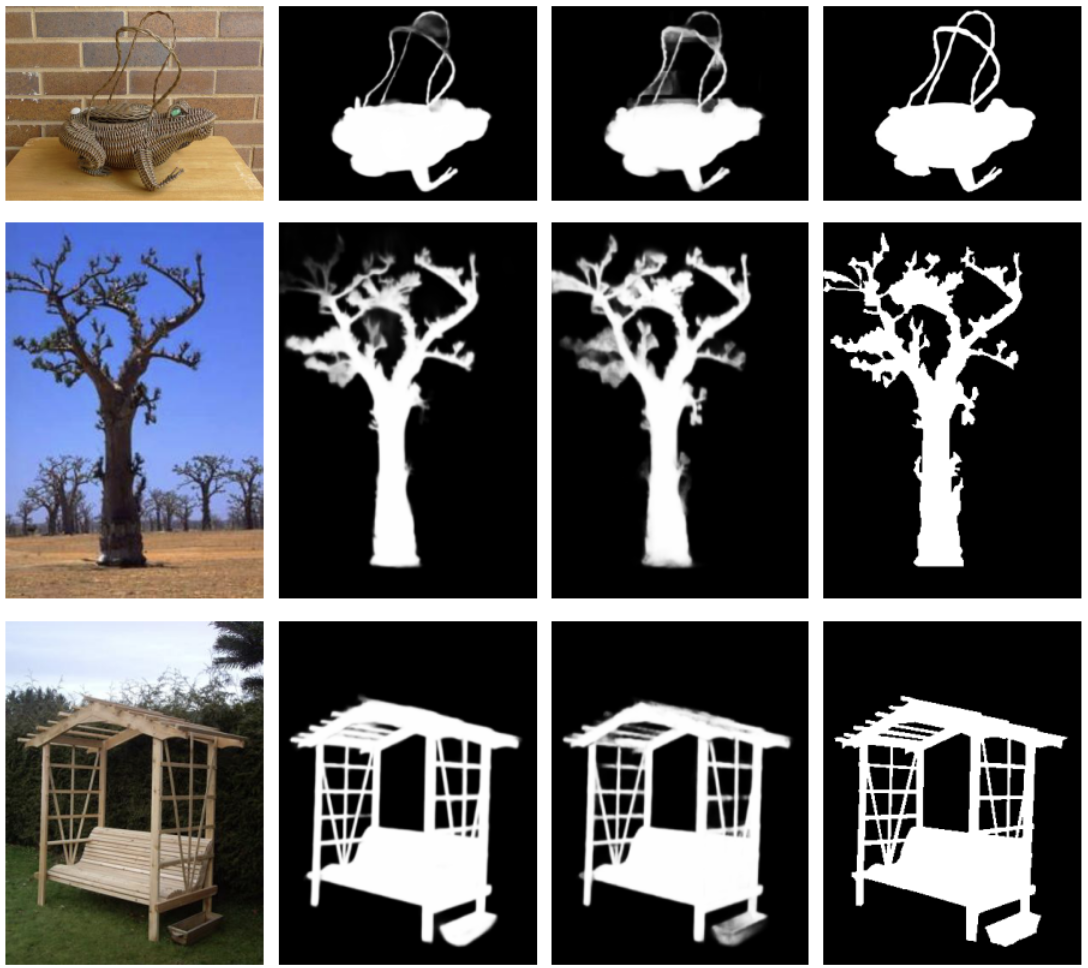
\includegraphics[width=0.7\textwidth]{img/Chapter2/OutputU2Net.png}
    \label{fig:output_u2net}
\end{figure}

\subsubsection{Công tác Lựa chọn và Làm Dữ liệu}
\begin{itemize}
    \item \textbf{Tập dữ liệu:}
    \begin{itemize}
        \item \textbf{Huấn luyện:} Sử dụng tập dữ liệu \textbf{DUTS-TR} (gồm 10,553 hình ảnh). Đây là tập dữ liệu lớn và thách thức nhất cho bài toán Salient Object Detection (SOD).
        \item \textbf{Kiểm thử:} Đánh giá trên 6 bộ benchmark phổ biến: \textbf{DUTS-TE, DUT-OMRON, HKU-IS, ECSSD, PASCAL-S, SOD}.
    \end{itemize}

    \item \textbf{Xử lý dữ liệu:}
    \begin{itemize}
        \item Multi-scale training với với hình ảnh được thay đổi kích thước thành 320×320 pixel.
        \item Mặt nạ nhị phân Ground truth được sử dụng để tính toán loss pixel theo pixel.
        \item Augmentation: mở rộng bao gồm lật ngang ngẫu nhiên và cắt ngẫu nhiên.
    \end{itemize}

    \item \textbf{Giao thức huấn luyện:}
    \begin{itemize}
        \item \textbf{Huấn luyện từ ban đầu:} Huấn luyện từ đầu không dùng backbone pre-trained.
        \item \textbf{Tối ưu:} Sử dụng SGD với learning rate $10^{-3}$, momentum 0.9, weight decay 0.0005.
        \item \textbf{Hàm mất mát:}
        \begin{equation}
        L_{total} = \sum_{d=1}^{6} w_d \cdot l_{side}^{(d)} + w_{fuse} \cdot l_{fuse} \quad (w=1.0)
        \end{equation}
    \end{itemize}
\end{itemize}

\subsubsection{Performance}
\textbf{Kết quả định lượng}
\begin{table}[H]
\centering
\caption{Thông số đo lường của $U^2$-Net trên các tập dữ liệu khác nhau (\cite{u2net_2020})}
\begin{tabular}{|l|c|c|c|c|c|}
\hline
\textbf{Tập dữ liệu huấn luyện} & \multicolumn{5}{l|}{DUTS-TR (10,553 ảnh)} \\ \hline
\textbf{Tối ưu} & \multicolumn{5}{l|}{SGD (lr $10^{-3}$, momentum 0.9, decay 0.0005)} \\ \hline
\textbf{Hàm mất mát} & \multicolumn{5}{l|}{Deep Supervision BCE (Trọng số mỗi tầng $w=1.0$)} \\ \hline
\hline
\textbf{Tập dữ liệu kiểm thử} & \textbf{$S_m \uparrow$} & \textbf{$F_{\beta}^{max} \uparrow$} & \textbf{$F_{\beta}^{\omega} \uparrow$} & \textbf{$E_m^{max} \uparrow$} & \textbf{MAE $\downarrow$} \\ \hline
DUTS-TE & 0.880 & 0.880 & 0.845 & 0.912 & 0.045 \\ \hline
DUT-OMRON & 0.826 & 0.808 & 0.752 & 0.854 & 0.054 \\ \hline
HKU-IS & 0.925 & 0.935 & 0.903 & 0.954 & 0.032 \\ \hline
ECSSD & 0.925 & 0.946 & 0.906 & 0.953 & 0.033 \\ \hline
PASCAL-S & 0.859 & 0.871 & 0.824 & 0.896 & 0.071 \\ \hline
SOD & 0.817 & 0.846 & 0.767 & 0.835 & 0.103 \\ \hline
\end{tabular}
\end{table}

\noindent \textbf{Đặc tính tính toán (đo trên GTX 1080Ti):} 
\begin{itemize}
    \item \textbf{$U^2$-Net (Full):} 176.3 MB, 44.0M tham số, 30 FPS.
    \item \textbf{$U^2$-Net$^\dagger$ (Small):} 4.7 MB, 0.7M tham số, 40 FPS.\\
\end{itemize}
\textbf{Điểm mạnh:} Cân bằng tốt giữa độ chính xác và hiệu quả, bảo toàn ranh giới tốt, kiến trúc gọn nhẹ.\\
\textbf{Điểm yếu:} Thời gian huấn luyện dài (600k vòng lặp), kiến trúc phức tạp.

\subsubsection{Đóng góp}
Phương pháp U\textsuperscript{2}-Net đóng góp chủ yếu vào Bước 2 và Bước 3 của saliency detection pipeline, tập trung vào việc học đặc trưng đa quy mô và mô hình hóa ngữ cảnh hiệu quả cho bài toán dense prediction.

\begin{itemize}
    \item \textbf{Cải tiến về trích xuất đặc trưng đa quy mô (multi-scale) trong cùng một tầng:} 
    Giới thiệu khối \textbf{RSU (ReSidual U-block)}, thực hiện một \textbf{U-structure nội bộ} để học đặc trưng ở nhiều quy mô \textbf{(intra-stage multi-scale)} mà vẫn giữ độ phân giải feature map, hạn chế mất chi tiết so với các backbone sâu (VGG/ResNet).
    \item \textbf{Cải tiến về mở rộng trường thụ cảm (receptive field) hiệu quả:}
    Thiết kế RSU giúp \textbf{mở rộng receptive field mạnh} trong khi số tham số \textbf{tăng tuyến tính}, từ đó tăng khả năng nắm bắt ngữ cảnh mà không làm mô hình phình to.
    \item \textbf{Cải tiến về mô hình hóa ngữ cảnh đa quy mô xuyên tầng:}
    Với kiến trúc \textbf{U-structure trong U-structure (Nested U-Net)}, mô hình học đồng thời \textbf{local details} và \textbf{global context} ở nhiều mức phân giải \textbf{(inter-stage multi-scale/context modeling)}.
\end{itemize}
\textbf{→ Cải thiện Bước 2 – Trích xuất đặc trưng.}

\begin{itemize}
    \item \textbf{Cải tiến về sinh saliency map biên sắc nét nhờ đặc trưng đa quy mô:}
    Việc kết hợp đặc trưng giàu ngữ cảnh (global) và chi tiết cục bộ (local) ở nhiều mức giúp decoder tái tạo saliency map với \textbf{ranh giới chính xác hơn} so với U-Net truyền thống.
    \item \textbf{Cải tiến về cân bằng độ chính xác và hiệu quả:}
    Thiết kế kiến trúc cho phép đạt chất lượng cao trong khi vẫn duy trì tính gọn nhẹ, bao gồm các biến thể nhỏ như U\textsuperscript{2}-Net$^\dagger$.
\end{itemize}
\textbf{→ Cải thiện Bước 3 – Sinh bản đồ nổi bật.}

\subsubsection{Hạn chế}
\begin{itemize}
    \item \textbf{Feature Refinement (Làm mịn đặc trưng):} Cấu trúc lặp lại nhiều lớp tích chập sâu, gặp khó khăn trong việc tách biệt các vật thể có độ tương phản cực thấp so với nền (low-contrast background). Đặc biệt là khi ranh giới giữa vật thể và nền bị nhòe, cơ chế trích xuất đặc trưng thuần túy của RSU đôi khi không đủ mạnh để "cắt" ranh giới sắc nét nếu không có thêm module Attention.
    \item \textbf{Độ phức tạp của giao thức huấn luyện:} Cần cấu hình và theo dõi kỹ lưỡng do huấn luyện từ đầu.
    \item \textbf{Khả năng mở rộng độ phân giải cao:} Yêu cầu bộ nhớ vẫn tăng theo kích thước ảnh do phải lưu trữ nhiều cấp độ đặc trưng.
    \item \textbf{Tốc độ  và tàu nguyên:} Dù số lượng tham số ít, nhưng số lượng phép tính (FLOPs) của $U^2$-Net vẫn tương đối lớn do cấu trúc lồng nhau phức tạp. Điều này khiến tốc độ xử lý trên CPU không thực sự ấn tượng so với các mô hình thuần túy tối ưu cho tốc độ.
\end{itemize}